\chapter[INTRODUÇÃO]{INTRODUÇÃO} \label{cap:introducao}

%\section{CONTEXTUALIZAÇÃO}
%, enquanto o gás natural gera a energia elétrica
%%contextualização  petróleo geral 


\begin{comment}
A Figura \ref{fig:bp2022} apresenta 3 gráficos das principais fontes energéticas mundiais, combustíveis fósseis (tais como, carvão mineral, gás natural e o petróleo), energias renováveis (tais como, solar, eólica, hidroelétrica, maremotriz) e elétrica. Cada gráfico apresenta três linhas, na cor verde representando um evolução conservadora, na cor laranja representando um crescimento acelerado e na cor azul representando uma evolução otimista. O eixo das ordenadas representa o percentual de participação na matriz energética, o eixo das abscissas varia de 2020 até 2050, a participação dos combustíveis fósseis apresenta uma tendência de redução até 2050, na perspectiva mais otimista essa redução pode chegar a 60\% e na mais conservadora pode atingir aproximadamente 30\%.
\begin{figure}[H]
    \centering
    \caption{Participação na matriz energética mundial }. 
    \label{fig:bp2022}
    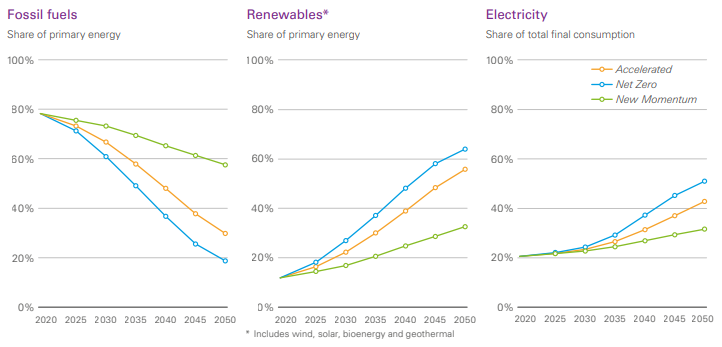
\includegraphics[width=160mm]{images/fig4.png}
    \fonte{\textit{British Petroleum Energy Outlook} \cite{bP2022}.}
\end{figure}
\end{comment}

%%petróleo Brasil - contexto atual 

O petróleo é a principal fonte de energia, fornecendo o combustível necessário para manter em funcionamento os diferentes meios de transporte \cite{gauto2016petroleo}. 
Após a pandemia de COVID, o valor do barril de petróleo se  manteve dentro da faixa de preços de US\$80 a US\$95, com início do conflito entre a Rússia e a Ucrânia o preço do barril de petróleo ultrapassou US\$140 \cite{ozili2022global}. 

De acordo com dados da Agência Nacional do Petróleo, Gás Natural e Biocombustíveis \cite{ANP2022}, a produção total de petróleo e gás natural no Brasil em abril de 2022 foi de 2,999 MMbbl/d (milhões de barris por dia) e 137 MMm3/d (milhões de metros cúbicos por dia), respectivamente. Essa produção foi proveniente de  6.089 poços, sendo 447 marítimos e 5.642 terrestres. A produção do pré-sal correspondeu a 75,4\% desse total e foi oriunda de 129 poços marítimos. Na Figura \ref{fig:Hu2018} apresenta um gráfico em colunas, o eixo das ordenadas presenta a quantidade em  MMbbl/d (milhões de barris por dia), o eixo da abcissas presenta o mês e ano da produção, os  dados mostram uma estabilidade na produção brasileira.

%%petróleo Brasil - descrição figura 2
\begin{figure}[H]
    \centering
    \caption{Histórico de produção de gás natural}. 
    \label{fig:Hu2018}
    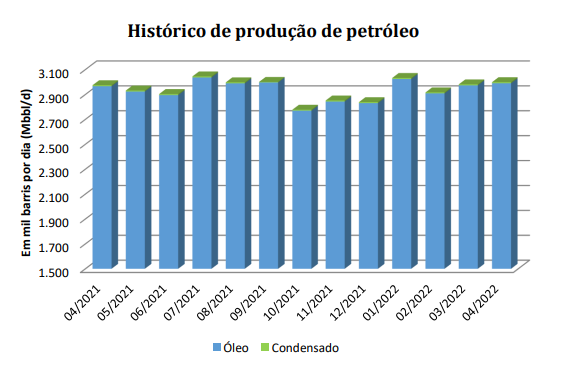
\includegraphics[width=130mm]{images/fig5.png}
    \fonte{Agência Nacional do Petróleo, Gás Natural e Biocombustíveis\cite{ANP2022}.}
\end{figure}

%%petróleo  - Anomalias  
Na industria do petróleo, é possível a ocorrência de eventos indesejados denominados anomalias. Por exemplo, o hidrato na linha de produção é uma anomalia, provocada pelo acúmulo de um composto cristalino formado por água e gás natural, que se assemelha a gelo  \cite{vargas2019base}, essa anomalia pode gerar perdas de produção durante dias ou até semanas, em alguns casos a desobstrução da linha é exigida, e a sonda marítima pode custar mais de 500 mil dólares ao dia \cite{andreolli2016introduccao}.  A detecção de anomalias é uma classificação do tipo binária (entre normalidade e anormalidade), na qual identifica-se a ocorrência de anomalia, porém sem especificá-la \cite{vargas2019base}.


%O monitoramento de processos industriais orientado a dados aplica estatísticas multivariadas e métodos de aprendizado de máquina para detectar e classificar anomalias em processos operacionais.
%% aprendizado de maquina
Na área de aprendizado de máquina, o problema de classificação pode ser definido como a categorização de uma determinada entrada em uma ou mais classes discretas e pré-definidas \cite{kadhim2019survey}. Em muitos processos industriais, busca-se detectar padrões raros, nos quais a maioria das observações referem-se a situações de normalidade, e a minoria, às situações raras que se deseja identificar \cite{santos2016literature}.



%% DESCRIÇÃO DO PROBLEMA 
\section{O PROBLEMA}

A indústria petrolífera possui um amplo monitoramento dos seus poços de petróleo, gerando assim uma grande quantidade de dados, esses dados estão disposto em MTS (do inglês \textit{Multivariate Time Series}, em português series temporais multivariadas) \cite{ismail2019deep}. Nas duas últimas décadas, a classificação de séries temporais tem sido considerada como um dos problemas mais desafiadores em mineração de dados.
O problema que motivou este trabalho é como detectar e classificar anomalias em poços petróleo por \textit{Multivariate Time Series}, em menor tempo de treinamento e com maior Acurácia do que os trabalhos correlatos identificados até o momento. 

Segundo \cite{rodrigo2021} o uso de técnica de redução de dimensão em problemas de detecção e classificação de anomalias em poços de produção de petróleo offshore apresentam resultados satisfatórios.

%% REDUÇÃO DE DIMENSIONALIDADE
No aprendizado de máquina, a alta dimensionalidade dos dados pode levantar problemas na precisão da classificação, reconhecimento de padrões e visualização. Treinamento em dados de alta dimensão podem se tornar difíceis devido à complexidade dos dados, o que pode levar ao que é chamado de maldição da dimensionalidade (do inglês,  \textit{Curse of Dimensionality}), como contramedida  muitas técnicas de redução de dimensionalidade foram propostas \cite{nanga2021review}.

\begin{comment}
\begin{figure}[H]
	\centering
	\caption{Plataforma de produção do pré-sal.}
	\label{fig:exemplo_sumarizacao_java}
	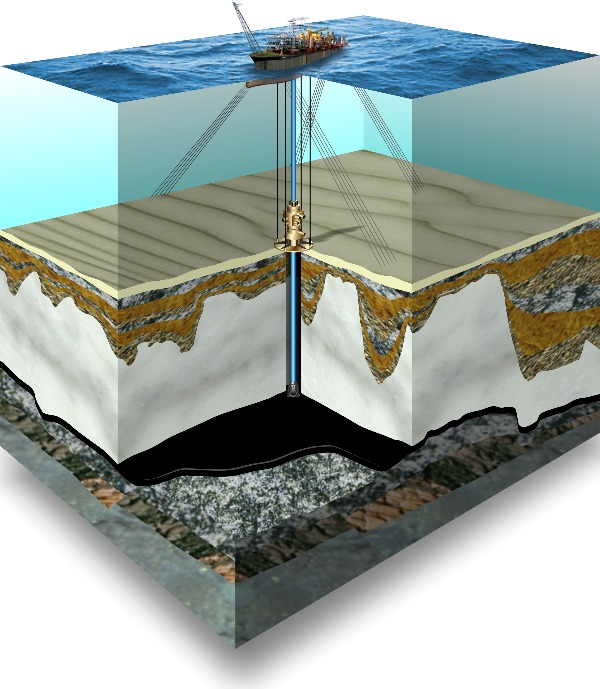
\includegraphics[width=105mm] 
	{images/plataforma.jpg}
	\fonte{Paulo Cabral/Banco de imagens da Petrobras.}
\end{figure}
\end{comment}

%% DESCRIÇÃO DA PROSPOSTA DO TRABALHO


\section{A PROPOSTA}
A hipótese deste trabalho é que aplicando técnicas de redução de dimensionalidade, podemos obter uma melhor acurácia do classificador do que a solução sem as técnicas de redução de dimensionalidade.

A proposta deste trabalho é utilizar três  técnicas de redução de dimensionalidade: KPCA (Análise de componentes principais do kernel, em inglês \textit {Kernel Principal Component Analysis}) \cite{nanga2021review}, ISOMAP (Mapeamento isométrico, em inglês \textit{Isometric Mapping}) \cite{jia2022iso}, e DMT (Transformação múltipla profunda , em inglês \textit{Deep Manifold Transformation}) \cite{li2020DTM}.

A base de dados a ser usada nos experimentos é a 3W \textit{dataset} \cite{vargas2019base}. Seguindo o trabalho de \citeonline{fernandes2022comparaccao} e \citeonline{junior2020detecccao}, serão usados os algoritmos de detecção de anomalias de classe única: Floresta de Isolamento (em inglês \textit{Isolation Forest}), Máquina de Vetor de Suporte de Classe Única (OCSVM do inglês, \textit{Oneclass Support Vector Machine}), Fator de Anomalia Local (LOF do inglês \textit{Local Outlier Factor}), Envelope Elíptico (MCD, do inglês \textit{Minimum Covariance Determinant}) e redes neurais do tipo \textit{Autoencoder} com camadas \textit{feedforward} e recorrentes do tipo LSTM (\textit{Long Short-Term Memory}). 

A métrica de comparação utilizada será  O F1-score é uma técnica simples que mede a discriminação de dois conjuntos de números reais\cite{F1akay2009support}, variando entre 0 e 1, Os resultados do uso de técnicas de redução de dimensionalidade serão comparados contra os resultados obtidos por  \citeonline{fernandes2022comparaccao} e \citeonline{junior2020detecccao}, que não usam esta etapa em sua solução.


%% DESCRIÇÃO DO PROBLEMA GERAL 
\section{OBJETIVO GERAL}
A ideia central da dissertação é a detecção de anomalias em poços de petróleo marítimos do tipo surgente, aplicando técnicas de redução de dimensionalidade.

%% DESCRIÇÃO DO OBJETIVOS 
\section{OBJETIVOS ESPECÍFICOS}
Para se alcançar o objetivo geral, os seguintes objetivos específicos serão realizados:
%% INICIO LISTA OBJETIVOS ESPECÍFICOS  
\begin{enumerate}

	\item {Realizar levantamento bibliográfico de trabalhos correlatos sobre Redução de dimensionalidade;}

	\item {Realizar levantamento bibliográfico sobre algoritmos de técnicas de redução de dimensionalidade }

	\item {Aplicar técnicas de redução de dimensionalidade:  KPCA (Análise de componentes principais do kernel, em inglês \textit {Kernel Principal Component Analysis}) \cite{nanga2021review}, ISOMAP (Mapeamento isométrico, em inglês \textit{Isometric Mapping}) \cite{jia2022iso}, e DMT (Transformação múltipla profunda , em inglês \textit{Deep Manifold Transformation}) \cite{li2020DTM}, ao 3W \textit{dataset}, para detecção de anomalias em poços de petróleo do tipo surgente;\cite{vargas2019base}}.
	
	\item {Aplicar técnicas detecção de anomalias de classe única:  Floresta de Isolamento (em inglês \textit{Isolation Forest}), Máquina de Vetor de Suporte de Classe Única (OCSVM do inglês, \textit{Oneclass Support Vector Machine}), Fator de Anomalia Local (LOF do inglês \textit{Local Outlier Factor}), Envelope Elíptico (MCD, do inglês \textit{Minimum Covariance Determinant}) e redes neurais do tipo \textit{Autoencoder} com camadas \textit{feedforward} e recorrentes do tipo LSTM (\textit{Long Short-Term Memory}} proposta por \cite{fernandes2022comparaccao}. 

    
    \item {Comparar os resultados obtidos após as utilização das técnicas de redução de dimensionalidade, com os resultados obtidos anteriormente por \cite{fernandes2022comparaccao}}, por meio da métrica F1-score .
    

\end{enumerate}
%% FIM  LISTA OBJETIVOS ESPECÍFICOS  


%% ORGANIZAÇÃO DO TRABALHO  
\section{ORGANIZAÇÃO DO TRABALHO}

Além deste capítulo introdutório, o restante deste documento está organizado em mais 3 capítulos. 
No Capítulo 2 será apresentado alguns trabalhos relacionados, sendo discutido as técnicas que foram utilizadas, os \textit{corpora} adotados e as medidas de avaliação para validar as propostas.
No Capítulo 3, será apresentada a proposta inicial deste trabalho, sendo discutido seus principais módulos e técnicas que serão exploradas.
Além disso, serão apresentados os corpora selecionados e as medidas de avaliação que serão adotadas para avaliar a abordagem proposta neste trabalho.
Por fim, no Capítulo 4, é apresentado o cronograma para execução do projeto de pesquisa.